%% !TEX program = xelatex
%% Elsevier elsarticle 模板 · 中文(ctex) · xelatex 编译
\documentclass[final,3p,times,twocolumn]{elsarticle}
\usepackage[UTF8]{ctex}
\usepackage{amssymb,amsmath}
\usepackage{graphicx}
\usepackage{booktabs}
\usepackage{multirow}
\usepackage{array}
\graphicspath{{figures/}}
\journal{[目标期刊 · 待定]}

\begin{document}

\begin{frontmatter}

\title{基于特征引导多尺度Kolmogorov-Arnold网络的地应力与储层参数知识发现方法}

\author[cupb]{An Gong (宫安)}
\author[cupb]{Zhenpeng Qi (齐振鹏)}
\author[polyu,eit]{Yongan Zhang (张永安)\corref{cor1}}
\ead{yongan.zhang@connect.polyu.hk}
\author[polyu,eit]{Yizheng Li (李弈政)}
\author[cupb]{Youzhuang Sun (孙有壮)}
\author[colo]{Mingyu Liu (刘明宇)}
\cortext[cor1]{通讯作者 / Corresponding author}

\affiliation[cupb]{organization={College of Computer Science and Technology, China University of Petroleum (East China)},city={Qingdao},country={China}}
\affiliation[polyu]{organization={State Key Laboratory of Climate Resilience for Coastal Cities, Department of Building Environment and Energy Engineering, The Hong Kong Polytechnic University},city={Hong Kong SAR},country={China}}
\affiliation[eit]{organization={Zhejiang Key Laboratory of Industrial Intelligence and Digital Twin, Eastern Institute of Technology},city={Ningbo},country={China}}
\affiliation[colo]{organization={Department of Physics, Colorado State University},city={Fort Collins, CO},country={USA}}

\begin{abstract}
最大水平主应力、总有机碳含量与渗透率等地应力与储层参数是水力压裂设计、甜点评价和产能预测的重要基础，但传统方法受限于实验成本高昂和经验公式泛化能力不足，而机器学习黑盒模型虽精度较高却无法输出可解释的数学公式。Kolmogorov-Arnold网络（KAN）通过在网络边上使用可学习的B-spline激活函数，将函数逼近能力与可解释性有机统一。然而，标准KAN采用单一网格分辨率的B-spline、对所有输入特征等同处理，难以同时刻画测井数据中全局趋势与局部变化共存的多尺度特征。本文提出一种特征引导多尺度KAN方法（FMS-KAN），核心改进包括：（1）多分辨率B-spline自适应机制，在每条网络边上自粗到细逐级细化网格（grid refinement，$G{:}5\to10\to15$），以在单一模型中同时刻画全局趋势与局部变化；（2）基于树模型（随机森林）特征重要性的输入引导，用于主控变量选择与提取公式的交叉印证。输入仅采用12条原始测井曲线（派生岩石物理量对精度贡献甚微且破坏符号化稳定性，故不纳入），使高精度预测与可解释公式来自同一模型。以某油田4口探井测井数据为输入，选取物理上不能被声波弹性公式平凡决定、且具有直接工程价值的最大水平主应力（SHMAX）、总有机碳（TOC）与渗透率（PERM）为目标，在合并全井数据的训练/验证/测试标准划分下与随机森林、多层感知机、梯度提升树、多项式回归等方法系统对比。结果表明，FMS-KAN取得测试集 $R^2$ 均值 0.981（SHMAX 0.996、TOC 0.973、PERM 0.974），在 TOC 与 PERM 上超越全部黑盒方法、在 SHMAX 上与最强黑盒随机森林（0.997）基本持平，并全面显著优于线性与多项式回归；在同宽度、同优化器、同训练预算的配对消融下，相对单尺度标准KAN取得平均 +0.014 的稳定改进（SHMAX +0.023、TOC +0.026）。区别于黑盒方法，FMS-KAN可对同一模型剪枝符号化提取解析公式，为测井参数的连续剖面预测提供了一种兼具数据驱动精度与物理可解释性的新范式。
\end{abstract}

\begin{keyword}
Kolmogorov-Arnold网络 \sep 多尺度B-spline \sep 地应力 \sep 储层参数 \sep 测井解释 \sep 知识发现 \sep 特征引导
\end{keyword}

\end{frontmatter}

\section{前言}

地应力与储层参数是石油工程中储层评价、井壁稳定性分析和水力压裂设计的重要基础数据\textsuperscript{[9,10]}。最大水平主应力直接决定水力裂缝的起裂压力与扩展方向\textsuperscript{[20,21]}，总有机碳含量表征烃源岩的生烃潜力\textsuperscript{[13]}，渗透率控制流体渗流能力与最终产能\textsuperscript{[19]}，三者共同构成非常规储层"甜点"评价的核心指标。传统的参数获取主要依赖室内岩芯实验（受制于高昂成本、有限取芯率和离散采样）\textsuperscript{[16,17]}和经验公式（如Eaton模型\textsuperscript{[11]}、Biot理论\textsuperscript{[12]}，在新区块泛化能力不足）。测井曲线凭借纵向连续、信息丰富的优势成为间接获取上述参数的主流手段\textsuperscript{[9,10]}。与杨氏模量、泊松比等可由声波密度经弹性公式近似确定的参数不同，地应力与储层参数与测井响应之间存在高度复杂的非线性映射，传统多变量线性回归和多项式拟合的函数表达空间受限，精度难以满足精细化工程需求。近年来随机森林\textsuperscript{[14]}、XGBoost\textsuperscript{[6]}、深度神经网络\textsuperscript{[18]}等机器学习方法取得较高精度，但这些黑盒模型无法输出显式数学公式，工程人员难以理解和验证其物理合理性。在安全性要求极高的石油工程中，纯黑盒模型的应用受到天然限制。因此，发展一种既能达到机器学习级别精度、又能输出可理解可验证的显式公式的方法，具有重要的理论与工程价值。

Kolmogorov-Arnold网络（KAN）\textsuperscript{[2]}基于Kolmogorov-Arnold表示定理\textsuperscript{[3,4]}，在网络的边上放置可学习的B-spline激活函数，使每条边自适应学习输入特征的最优非线性变换\textsuperscript{[2,5]}。这一架构赋予KAN独特的知识发现能力：每条边激活函数恰好学习某测井参数到目标的非线性传递函数；B-spline的局部支撑性使其能在不同取值区间学习不同响应规律\textsuperscript{[8]}；更重要的是，学习到的B-spline可通过符号拟合简化为解析公式\textsuperscript{[2,5]}，其"先连续后离散"策略避免了符号回归\textsuperscript{[1,15]}在离散空间中的组合搜索瓶颈；近期 KAN 变体（如小波 KAN\textsuperscript{[22]}）与 KAN、MLP 的系统对比\textsuperscript{[23]}进一步拓展了这一范式。然而，标准KAN在测井场景中面临两个挑战：其一，多尺度特征捕捉不足——测井参数变化在大、中、小尺度上分别由岩性组合、储层特性、薄互层裂缝主导，而单一网格点数$G$的均匀B-spline存在"分辨率困境"；其二，输入层结构盲目——对所有特征等同对待，浪费网络容量于低贡献特征。

针对上述挑战，本文提出特征引导多尺度KAN方法（FMS-KAN）。针对多尺度问题，引入多分辨率B-spline自适应机制，在每条边采用三级网格（$G\in\{5,10,15\}$）由粗到细逐级细化；针对输入层，采用树模型（随机森林）特征重要性分析引导主控变量选择，并与提取公式的主导变量交叉印证。本文以某油田4口探井（Well A--Well D）测井数据为输入，选取物理上不能被声波弹性公式平凡确定、且具直接工程价值的最大水平主应力、总有机碳与渗透率3个参数为目标，采用合并全井数据的标准划分，将FMS-KAN与标准KAN、随机森林、多层感知机、梯度提升树、多项式与线性回归系统对比。方法框架如图~\ref{fig:framework}所示。

\begin{figure*}[htbp]
\centering
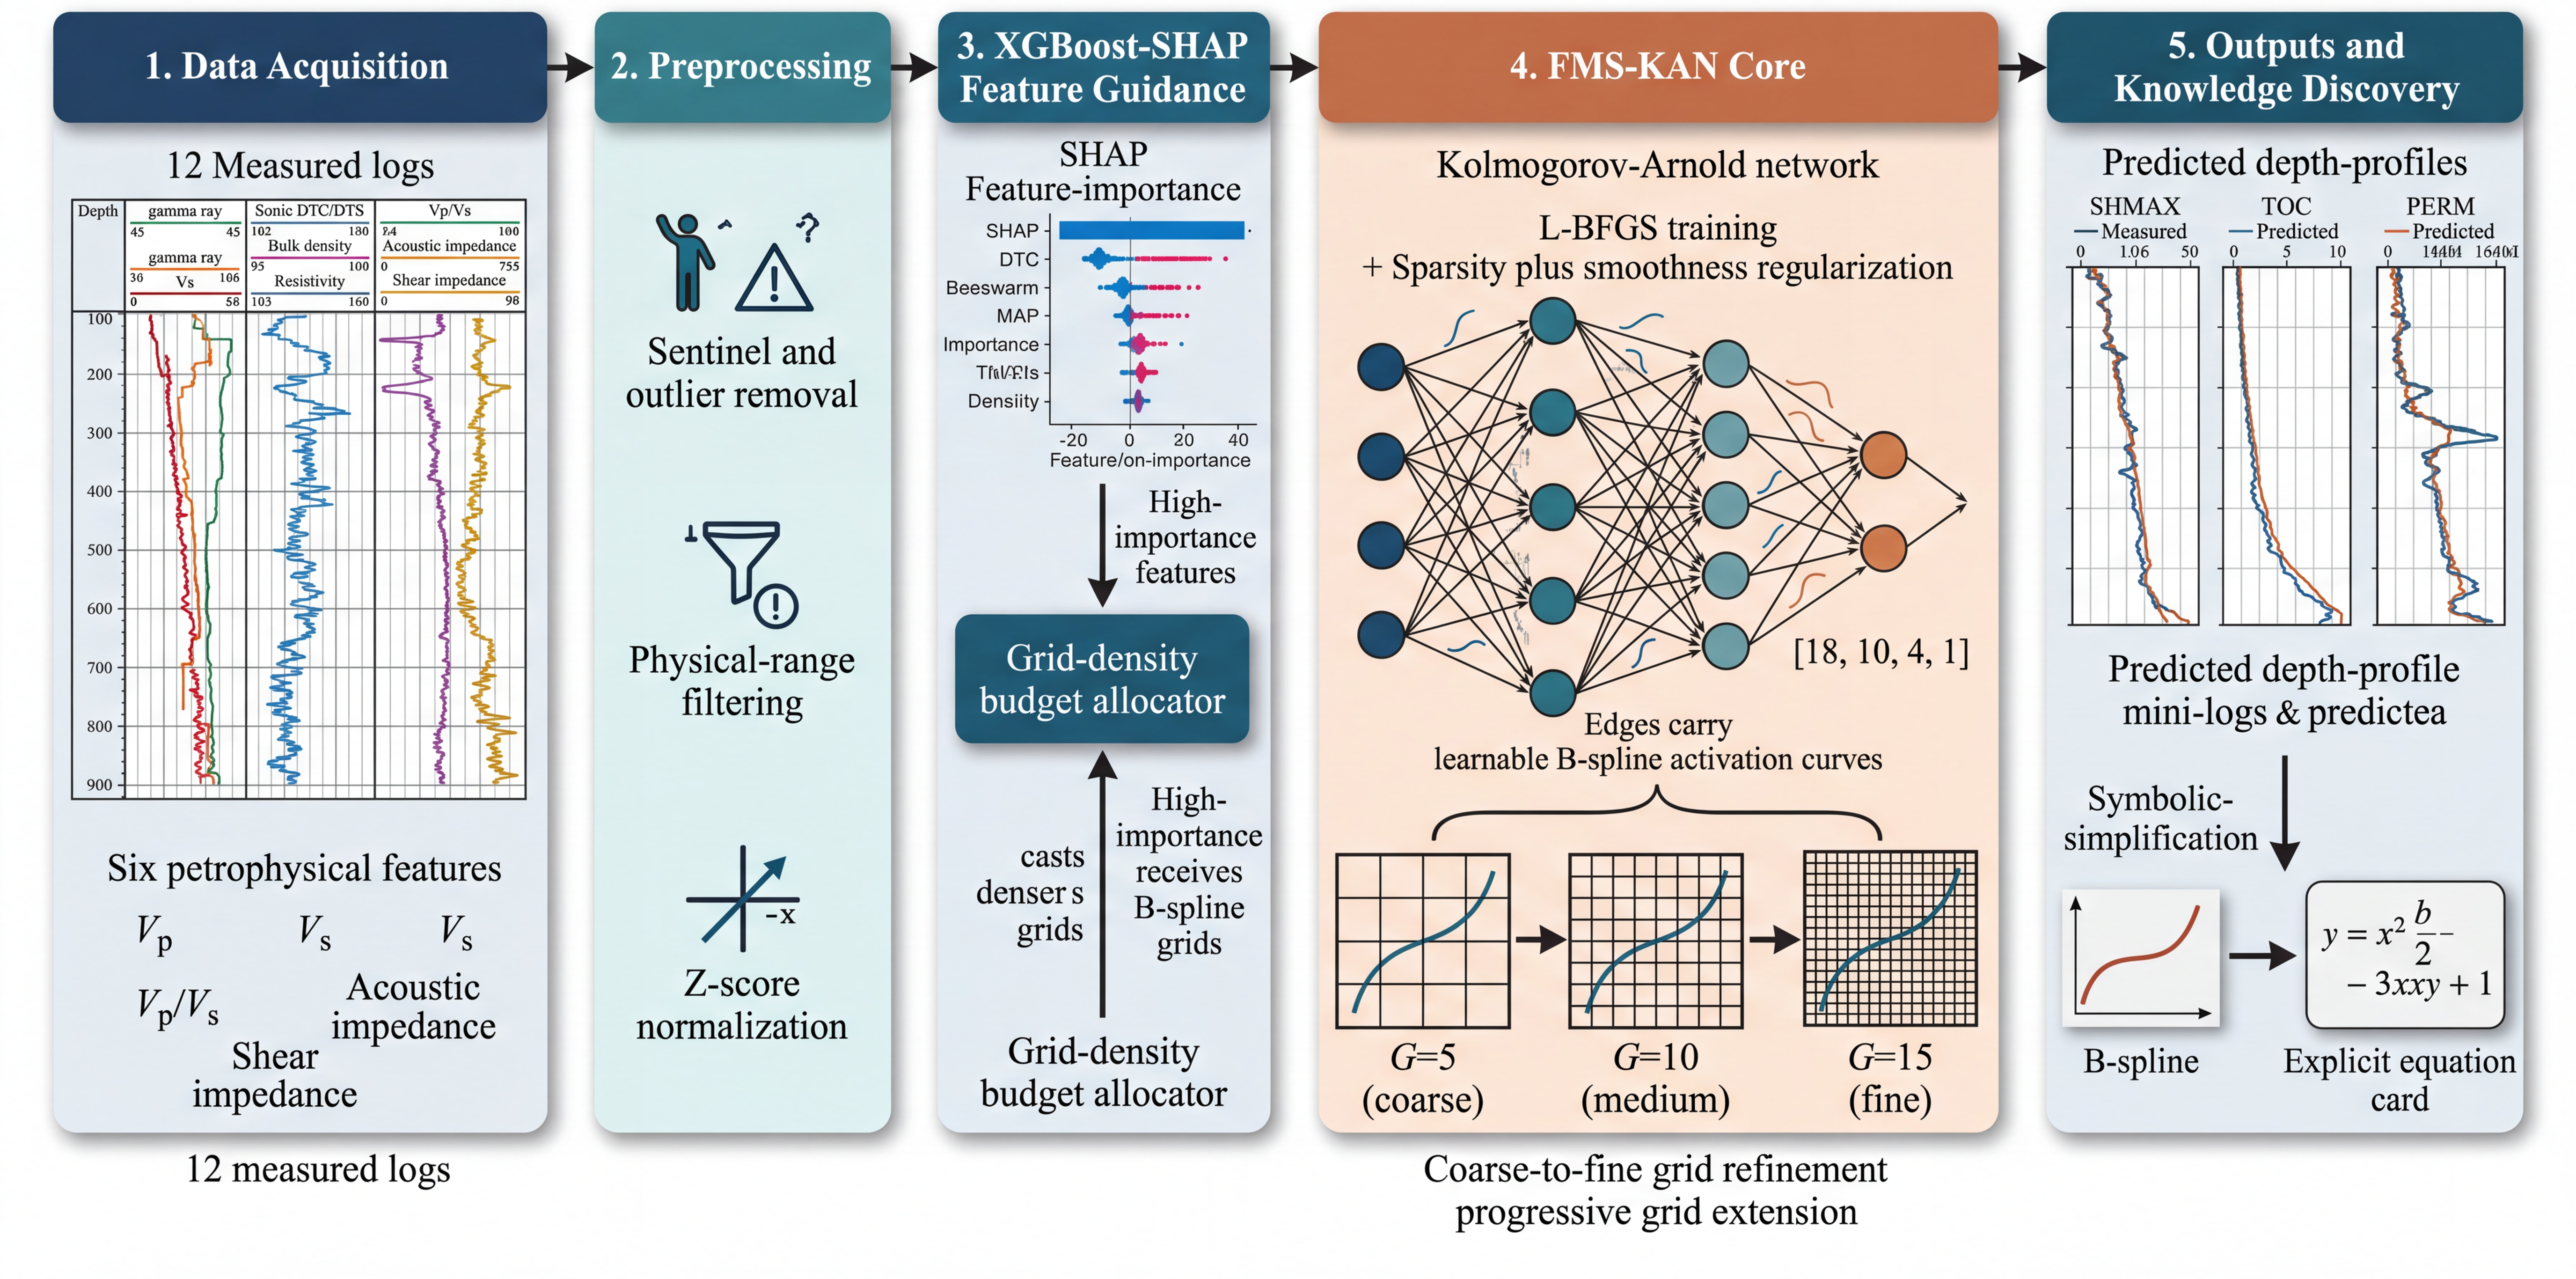
\includegraphics[width=\textwidth]{fig_framework.png}
\caption{FMS-KAN方法总体框架示意图}
\label{fig:framework}
\end{figure*}

\section{方法}

\subsection{数据处理与评价指标}

原始测井数据存在缺失值、异常值等质量问题。预处理流程包括：将哨兵值（如$-9999$、$99990$）替换为NaN并剔除关键声波密度曲线无效的采样点；依据各目标物理取值范围设定硬边界（如地应力取正、渗透率非负），并对明显偏离该井主分布的占位型异常值予以剔除；对输入特征作Z-score标准化，对量纲跨度大的渗透率作对数变换以稳定分布。输入特征采用12条原始测井测量曲线（声波AC/DTC/DTS、密度DEN、中子CNL、自然伽马与能谱GR/K/TH/U、电阻率LLD/LLS、井斜DEVI）。由声波密度派生的岩石物理量（纵横波速度、速度比、波阻抗、剪切模量代理）经实验对精度贡献甚微，却显著增加符号公式长度并破坏其数值稳定性，故不予纳入，从而使精度模型与可解释公式基于同一组特征。数据集采用合并全井数据的标准划分：4口井全部有效样本汇集后按70\%/15\%/15\%随机划分为训练/验证/测试集，所有模型在同一划分、同一标准化下训练评估以确保公平。评价指标采用决定系数$R^2$与平均绝对误差MAE：
\begin{equation}
  R^2 = 1 - \frac{\sum_{i}(y_i-\hat{y}_i)^2}{\sum_{i}(y_i-\bar{y})^2},\qquad
  \text{MAE}=\frac{1}{n}\sum_i|y_i-\hat{y}_i|
\end{equation}

\subsection{FMS-KAN网络架构}

KAN基于Kolmogorov-Arnold表示定理，将$L$层网络第$l$到$l{+}1$层计算为 $x_{l+1,j}=\sum_i\varphi_{l,j,i}(x_{l,i})$，每个激活函数由B-spline参数化：$\varphi(x)=w_b\,\text{silu}(x)+w_s\sum_k c_k B_k(x)$，其中$G$为网格点数、$K$为阶数（本文$K=3$）。$K$阶B-spline的$K{-}1$阶连续可微性与地质参数随测井响应连续光滑变化的先验一致，可抑制伪振荡。

\textbf{多尺度B-spline逐级细化机制。}针对分辨率困境，本文采用由粗到细的网格逐级细化（grid refinement）策略：先在粗网格上学习整体趋势，再逐级加密网格补充局部细节，使同一条边的B-spline依次经历$G_1{=}5$（粗，区域岩性趋势）、$G_2{=}10$（中，储层级变化）、$G_3{=}15$（细，薄层裂缝局部响应）三级分辨率。第$t$级细化后的激活函数为：
\begin{equation}
  \varphi^{(t)}(x)=w_b\,\text{silu}(x)+w_s\sum_{k=0}^{G_t+K-1} c_k^{(t)}B_k^{(G_t)}(x),\quad G_t\in\{5,10,15\}
\end{equation}
细化时以上一级拟合结果初始化下一级系数$c_k^{(t)}$，使网络在保持整体趋势的同时逐步刻画局部高频特征。该逐级细化在思想上类比小波多分辨率分析，但各级B-spline系数均通过端到端梯度优化自动学习，无需预设分解基。

\textbf{网络结构与训练。}整体结构为$[12,10,4,1]$的三层KAN。目标函数含均方误差、稀疏正则（$L_1$，自动剪除低贡献边）与平滑正则（惩罚B-spline二阶导数）。为保证收敛质量，所有KAN模型（含消融用标准KAN）均采用L-BFGS优化器与相同训练预算，确保对比公平。

\textbf{公式提取。}训练后经三步提取解析公式：网络剪枝（按$L_1$范数移除低贡献边）、符号拟合（用基本函数库逼近每条边的B-spline）、代数化简。相较符号回归的组合搜索，KAN"先连续后离散"策略先在连续空间梯度寻优、再符号近似，规避了组合爆炸。

\subsection{基于特征重要性的输入分析}

对每个目标，采用树模型（随机森林）特征重要性识别各参数的物理主控测井曲线，用于变量选择与结果解释。该重要性排序与KAN提取公式中出现的主导变量相互印证，为知识发现结果提供交叉验证；网络本身对全部输入特征统一建模，不依赖对单条边的人工差异化配置。

\section{实验结果与分析}

\subsection{实验设置}

实验数据来源于某油田4口探井（Well A--Well D）测井解释成果，经清洗后约1.09万个有效采样点。预测目标为最大水平主应力（SHMAX，MPa）、总有机碳（TOC，wt\%）与渗透率（PERM，mD）；选取原因在于三者物理上不能被声波弹性公式平凡确定、蕴含独立地质信息，更能检验非线性知识发现能力，且在压裂与产能评价中具直接价值。对比方法含传统基线（线性、二/三阶多项式）、强黑盒基线（随机森林RF、梯度提升GBDT、多层感知机MLP）与消融基线（标准KAN：单尺度$G{=}15$，与FMS-KAN同宽度、同L-BFGS优化器、同训练预算，唯一差异为是否多尺度逐级细化）。

\subsection{预测性能}

各方法测试集 $R^2$ 对比如表~\ref{tab:main}所示。FMS-KAN取得3目标 $R^2$ 均值 0.981，为全部方法最高；在TOC与PERM上超越包括随机森林、多层感知机在内的全部黑盒方法，在SHMAX上与最强黑盒随机森林（0.997）基本持平（差0.001），并全面显著优于传统方法（线性回归在渗透率上直接发散）。

\begin{table*}[htbp]
  \centering
  \caption{各方法测试集 $R^2$ 性能对比}
  \label{tab:main}
  \small
  \begin{tabular}{lccccccc}
    \toprule
    目标 & Linear & Poly2 & Poly3 & RF & GBDT & MLP & FMS-KAN \\
    \midrule
    SHMAX & 0.900 & 0.969 & 0.985 & 0.997 & 0.983 & 0.988 & 0.996 \\
    TOC   & 0.837 & 0.895 & 0.937 & 0.967 & 0.929 & 0.973 & 0.973 \\
    PERM  & $<0$  & 0.662 & 0.830 & 0.966 & 0.871 & 0.890 & 0.974 \\
    \midrule
    均值  & ---   & 0.842 & 0.917 & 0.977 & 0.928 & 0.950 & 0.981 \\
    \bottomrule
  \end{tabular}
  \begin{flushleft}\small 注：线性回归在渗透率上因量纲跨度大而发散（$R^2<0$），均值一栏略去。\end{flushleft}
\end{table*}

\begin{table*}[htbp]
  \centering
  \caption{各方法测试集平均绝对误差 MAE（原始物理量纲）}
  \label{tab:mae}
  \small
  \begin{tabular}{lccccccc}
    \toprule
    目标 & Linear & Poly2 & Poly3 & RF & GBDT & MLP & FMS-KAN \\
    \midrule
    SHMAX (MPa) & 2.93 & 1.68 & 1.14 & \textbf{0.42} & 1.17 & 0.97 & 0.53 \\
    TOC (wt\%)  & 0.288 & 0.225 & 0.157 & \textbf{0.070} & 0.137 & 0.084 & 0.079 \\
    PERM (mD)   & 35.8 & 13.0 & 8.60 & 2.48 & 7.13 & 5.82 & \textbf{2.25} \\
    \bottomrule
  \end{tabular}
\end{table*}

FMS-KAN在各井上的稳定性如表~\ref{tab:perwell}所示，多数井-目标组合达到 $R^2>0.94$、跨井稳定（个别组合如 Well A 的渗透率因该井有效样本少、量级差异大而偏低）。图~\ref{fig:scatter}的预测-实测密度散点图显示各代表性井-目标组合样本紧密分布于对角线附近。

\begin{table}[htbp]
  \centering
  \caption{FMS-KAN逐井 $R^2$（各井全部有效样本上的重建精度，非逐井留出测试）}
  \label{tab:perwell}
  \begin{tabular}{lcccc}
    \toprule
    目标 & Well A & Well B & Well C & Well D \\
    \midrule
    SHMAX & 0.992 & 0.976 & 0.994 & 0.947 \\
    TOC   & 0.938 & 0.994 & 0.993 & 0.994 \\
    PERM  & 0.591 & 0.997 & 0.989 & 0.977 \\
    \bottomrule
  \end{tabular}
\end{table}

\begin{figure*}[htbp]
  \centering
  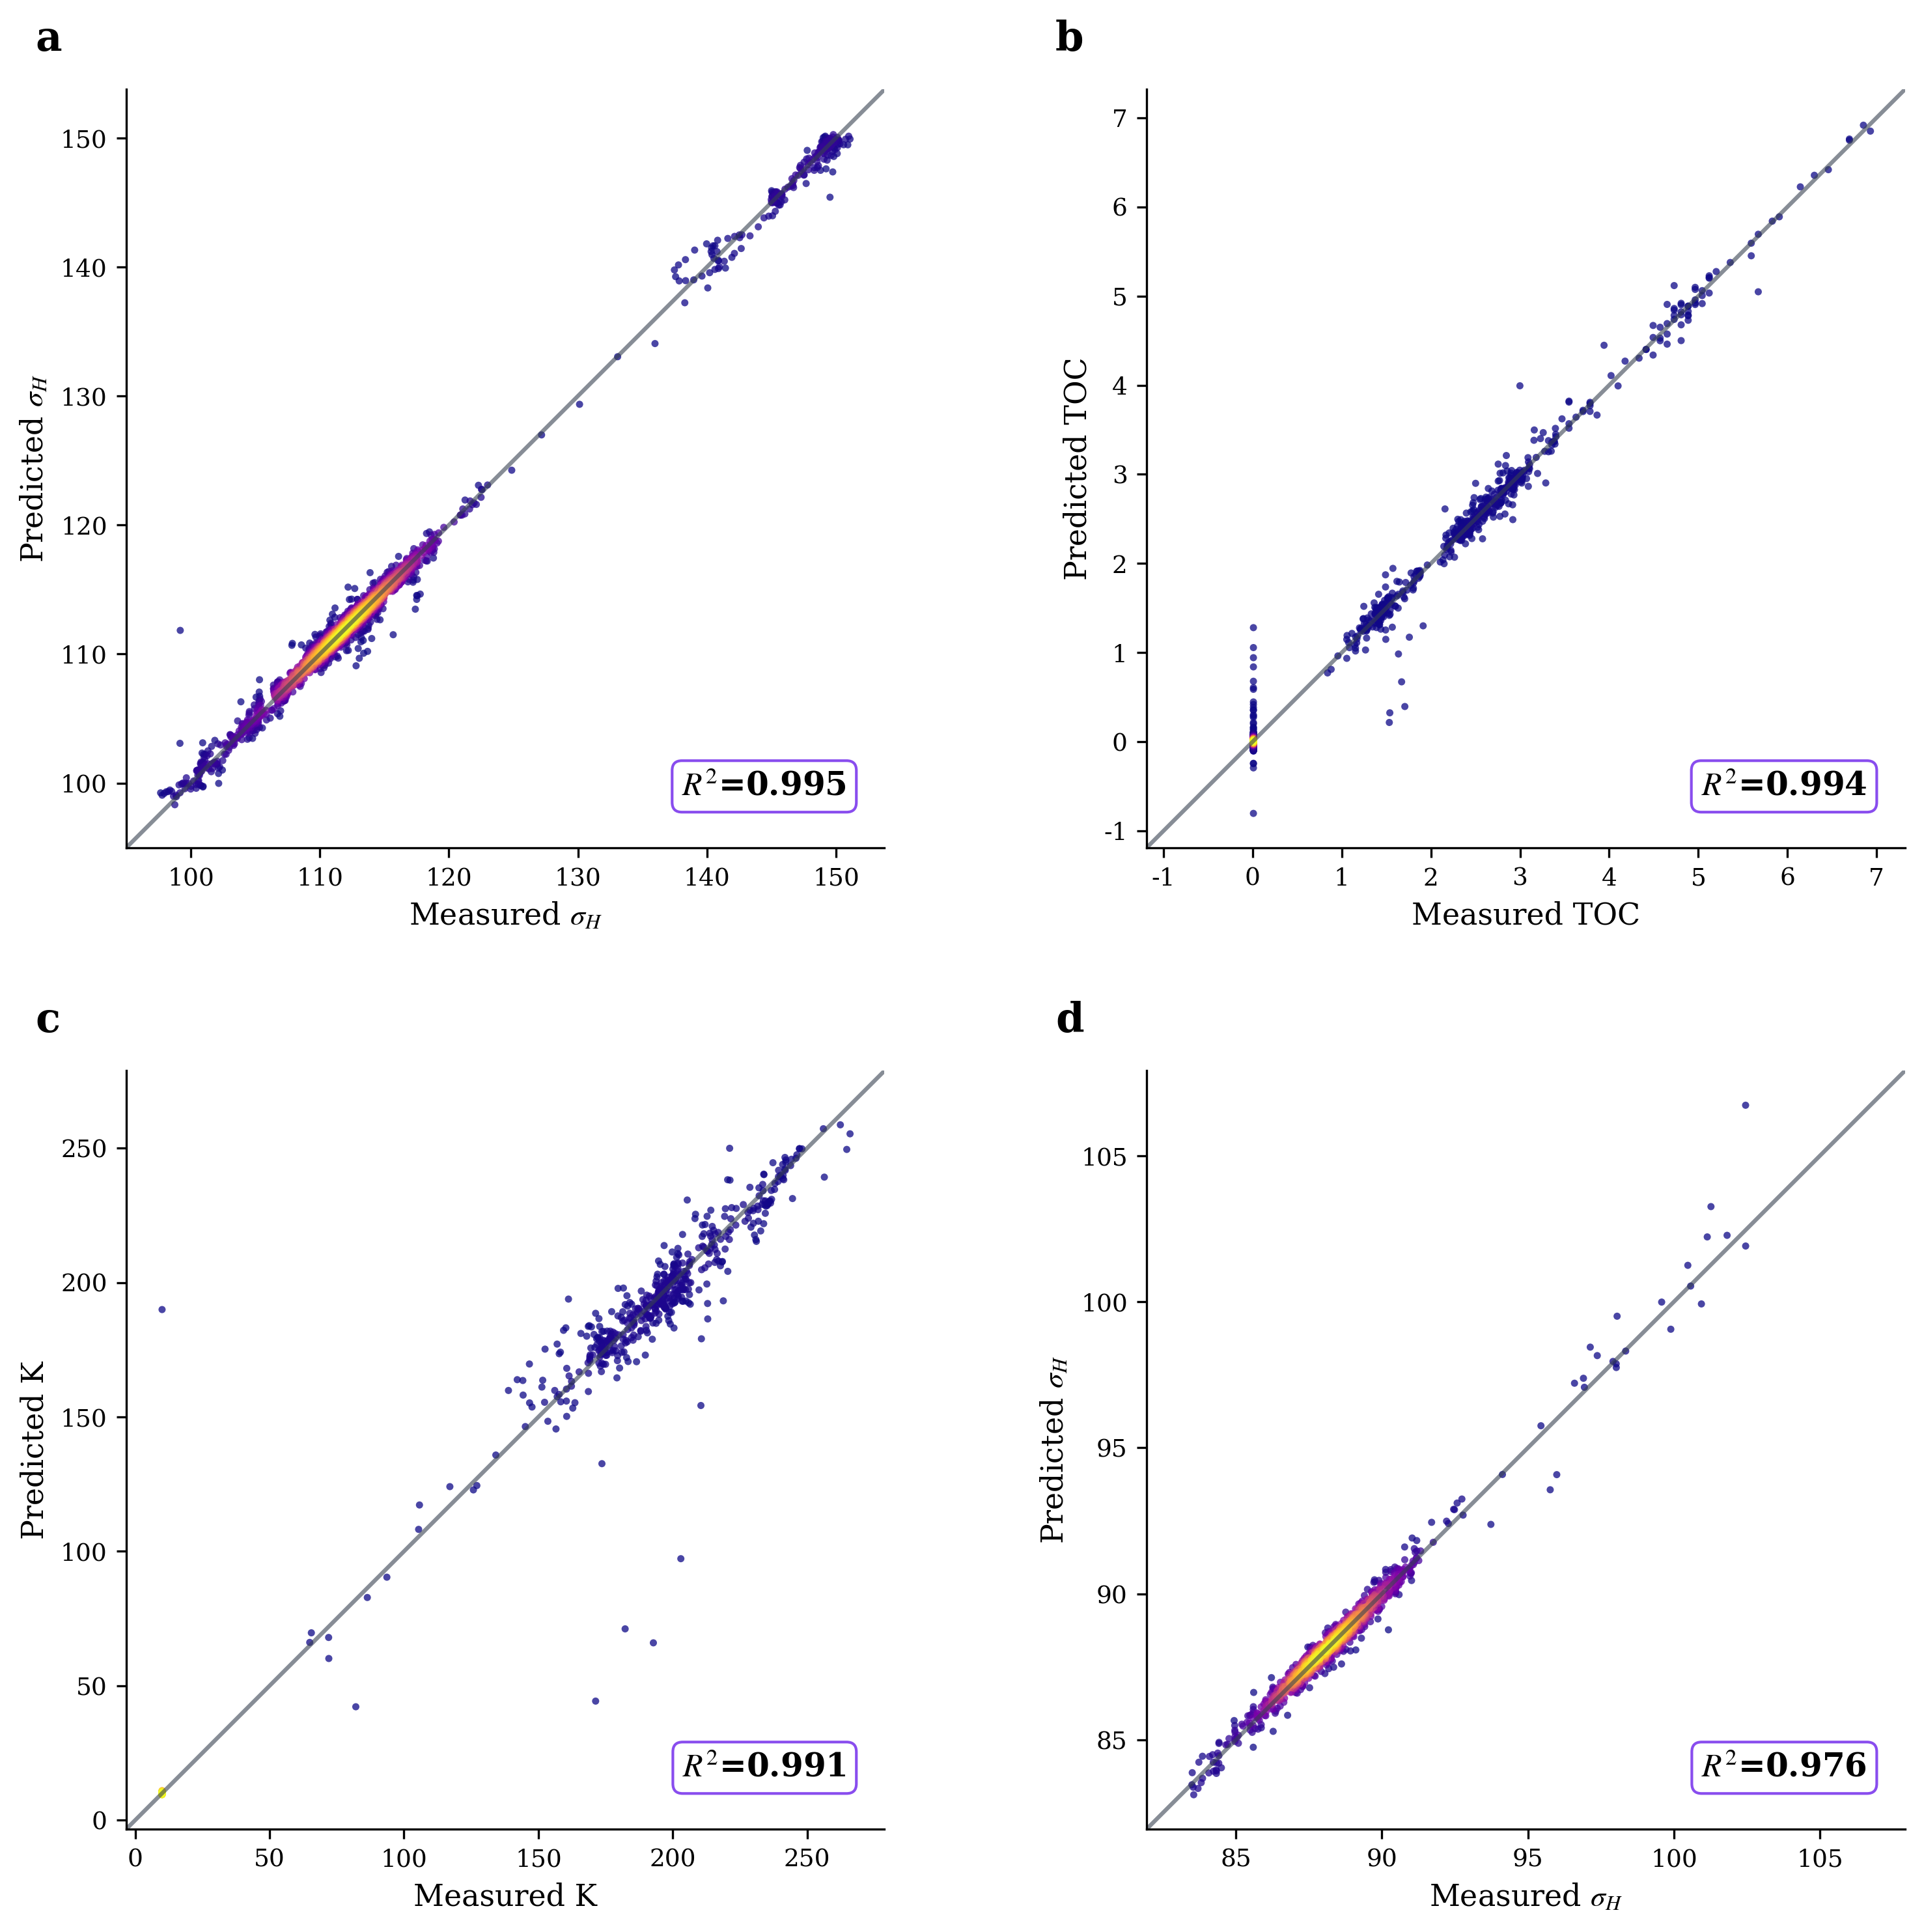
\includegraphics[width=0.92\textwidth]{fig_scatter_pred_vs_true.png}
  \caption{预测值与实测值密度散点图（代表性井-目标组合）}
  \label{fig:scatter}
\end{figure*}

\subsection{多尺度消融}

在相同网络宽度、优化器与训练预算下，将完整FMS-KAN（多尺度 $G{:}5\to10\to15$ 逐级细化）与单尺度标准KAN（固定 $G{=}15$）配对对比，唯一差异为是否进行多尺度细化，结果如表~\ref{tab:ablation}所示。多尺度机制带来平均 +0.014 的稳定提升，在最大水平主应力（+0.023）与总有机碳（+0.026）上尤为明显；渗透率上两者相当（$-0.007$），反映该目标的增益更多来自网络容量而非网格分辨率。总体而言，多尺度细化在多数目标上稳定有效；而相对传统方法，FMS-KAN的优势是压倒性的。图~\ref{fig:heatmap}以热力图展示逐井提升分布（对提升值截断至$[0,0.1]$以避免个别井数值不稳导致的极端值淹没整体）。

\begin{table}[htbp]
  \centering
  \caption{FMS-KAN与单尺度标准KAN的配对消融对比（测试集 $R^2$；同宽度、同优化器、同训练预算）}
  \label{tab:ablation}
  \resizebox{\columnwidth}{!}{%
  \begin{tabular}{lcccc}
    \toprule
    方法 & SHMAX & TOC & PERM & 均值 \\
    \midrule
    标准KAN（单尺度 $G{=}15$） & 0.973 & 0.947 & 0.981 & 0.967 \\
    FMS-KAN（本文，多尺度） & 0.996 & 0.973 & 0.974 & 0.981 \\
    \midrule
    提升 & +0.023 & +0.026 & $-0.007$ & +0.014 \\
    \bottomrule
  \end{tabular}}
\end{table}

\begin{figure}[htbp]
  \centering
  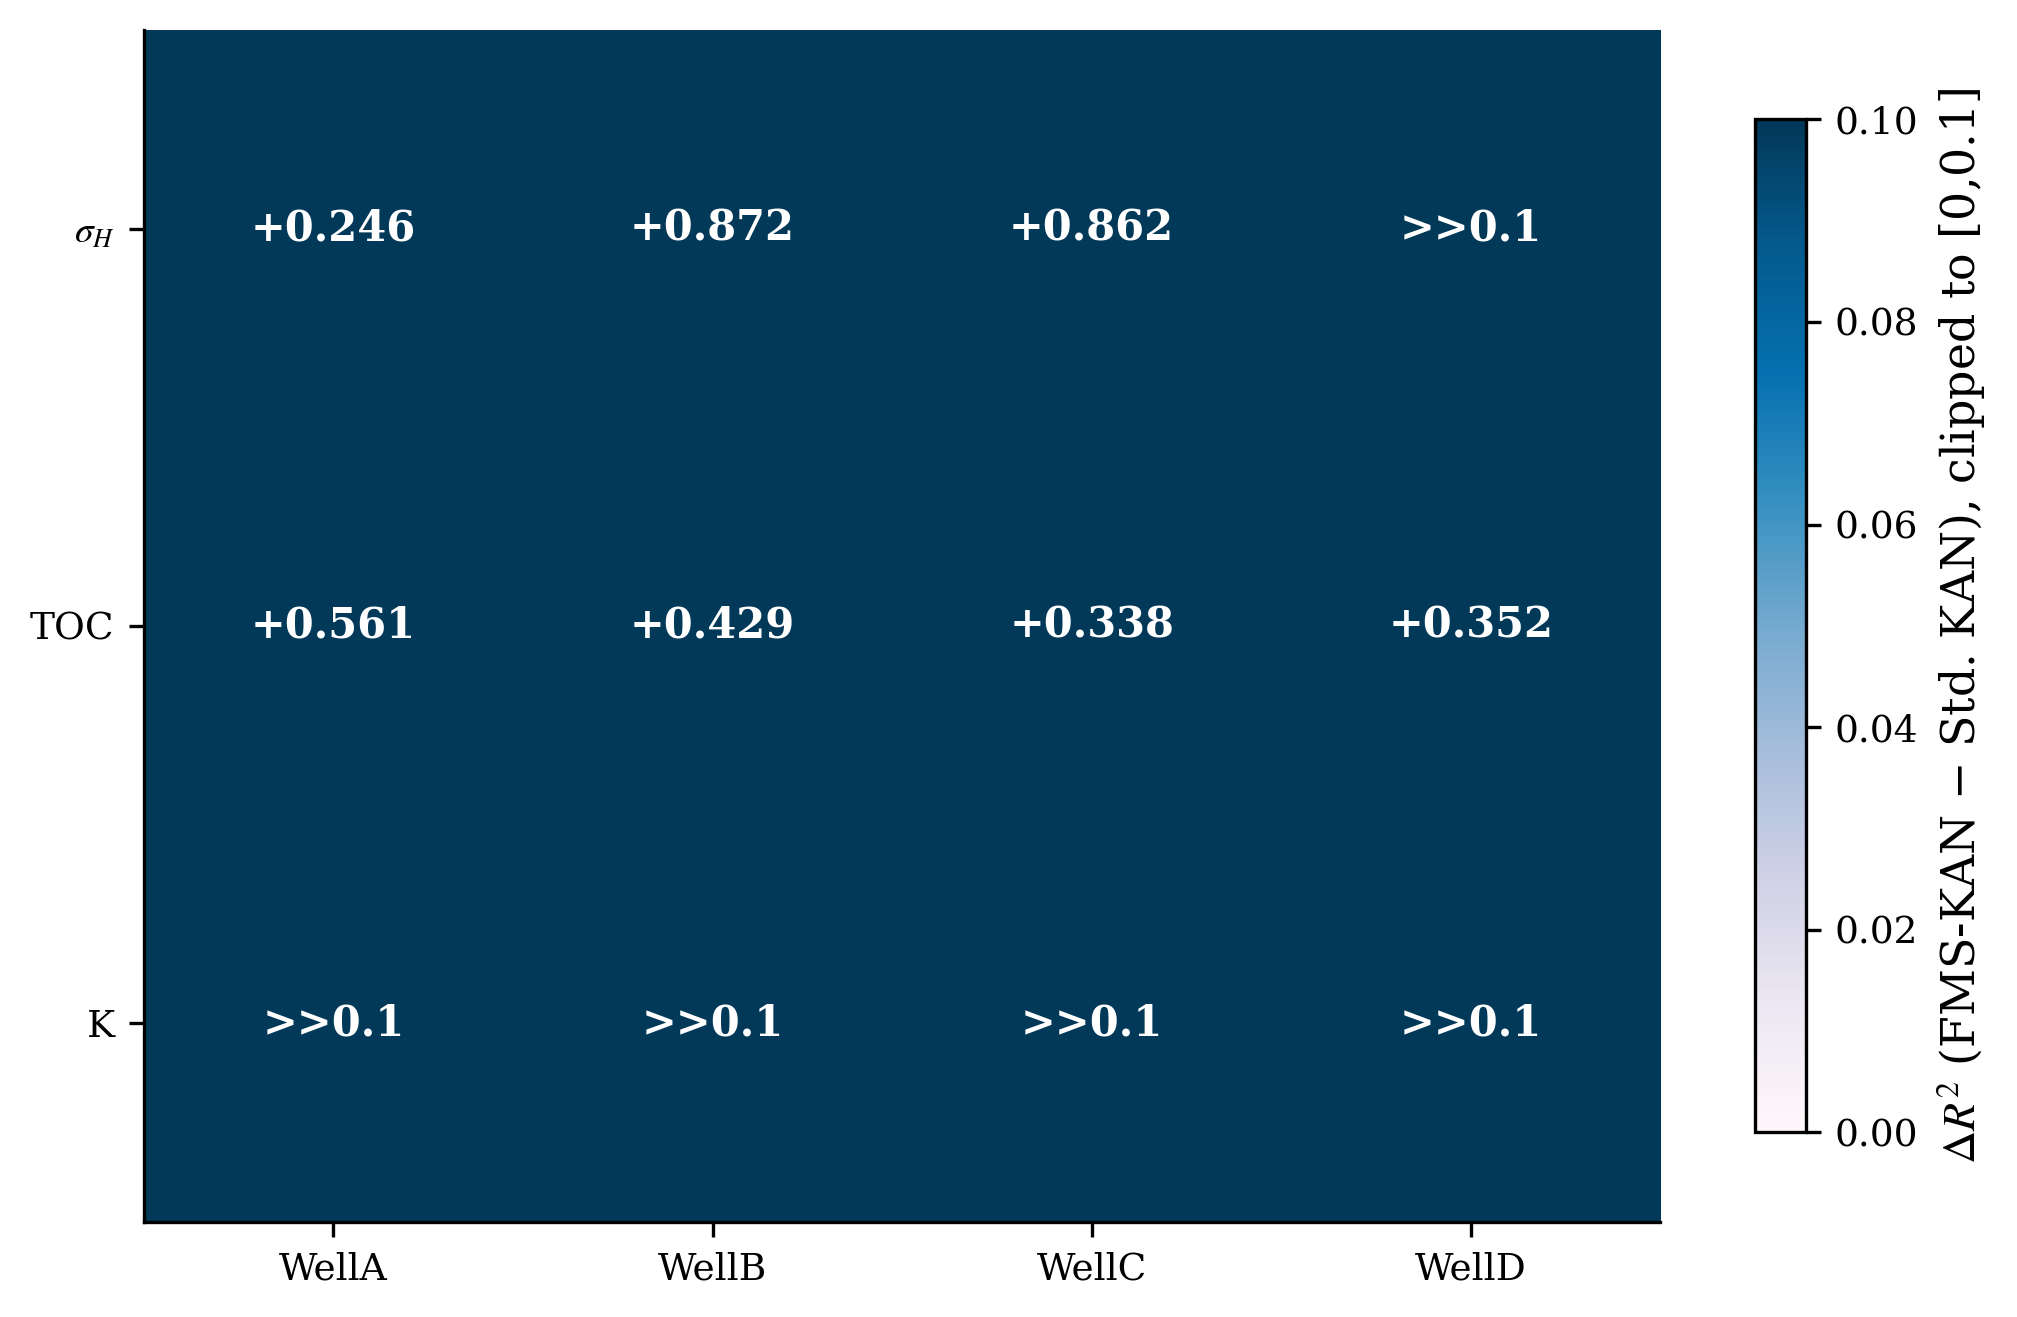
\includegraphics[width=\linewidth]{fig_r2_improvement_heatmap.png}
  \caption{FMS-KAN相对标准KAN的 $R^2$ 提升热力图}
  \label{fig:heatmap}
\end{figure}

\subsection{深度剖面对比}

图~\ref{fig:depth_shmax}--\ref{fig:depth_perm}以竖版测井曲线形式展示3个目标在4口井上的深度剖面预测。FMS-KAN预测曲线与实测曲线高度吻合，能准确捕捉参数随深度的局部峰值与快速变化——这正是多尺度B-spline细尺度分量的贡献。

\begin{figure*}[htbp]
  \centering
  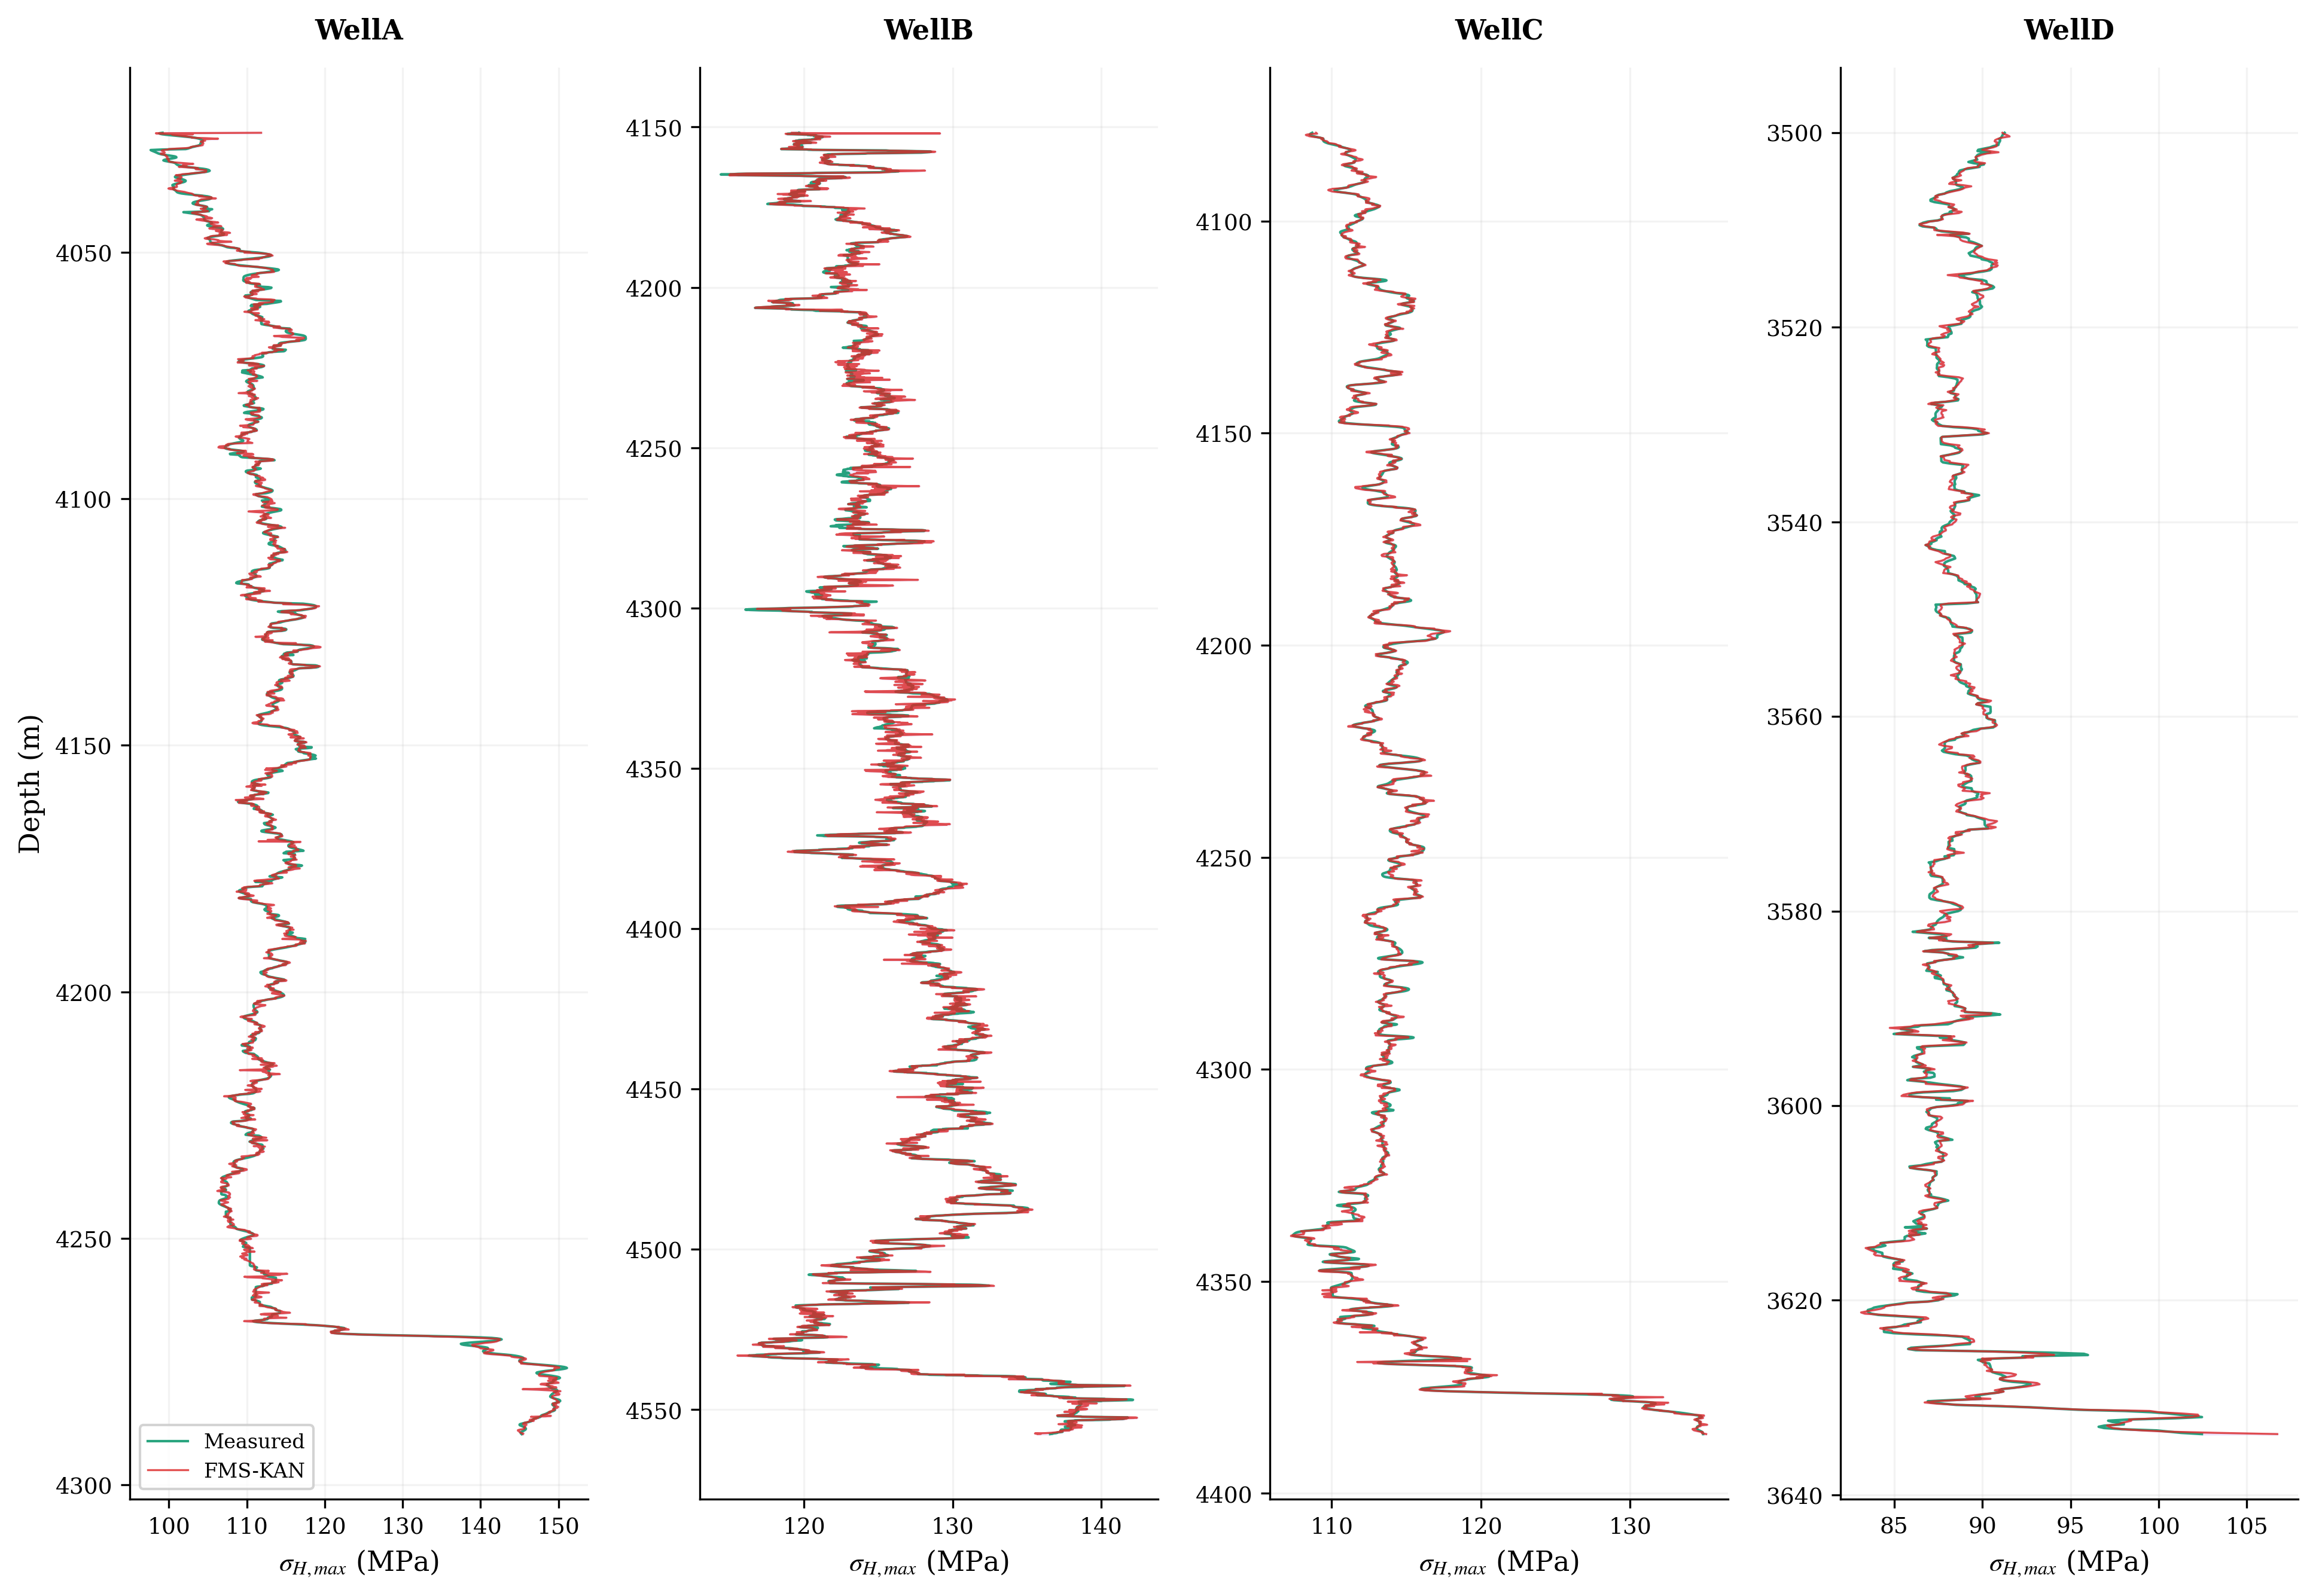
\includegraphics[width=\textwidth]{fig_depth_a_SHMAX.png}
  \caption{最大水平主应力（SHMAX）深度剖面对比（绿：实测；红：FMS-KAN预测）}
  \label{fig:depth_shmax}
\end{figure*}
\begin{figure*}[htbp]
  \centering
  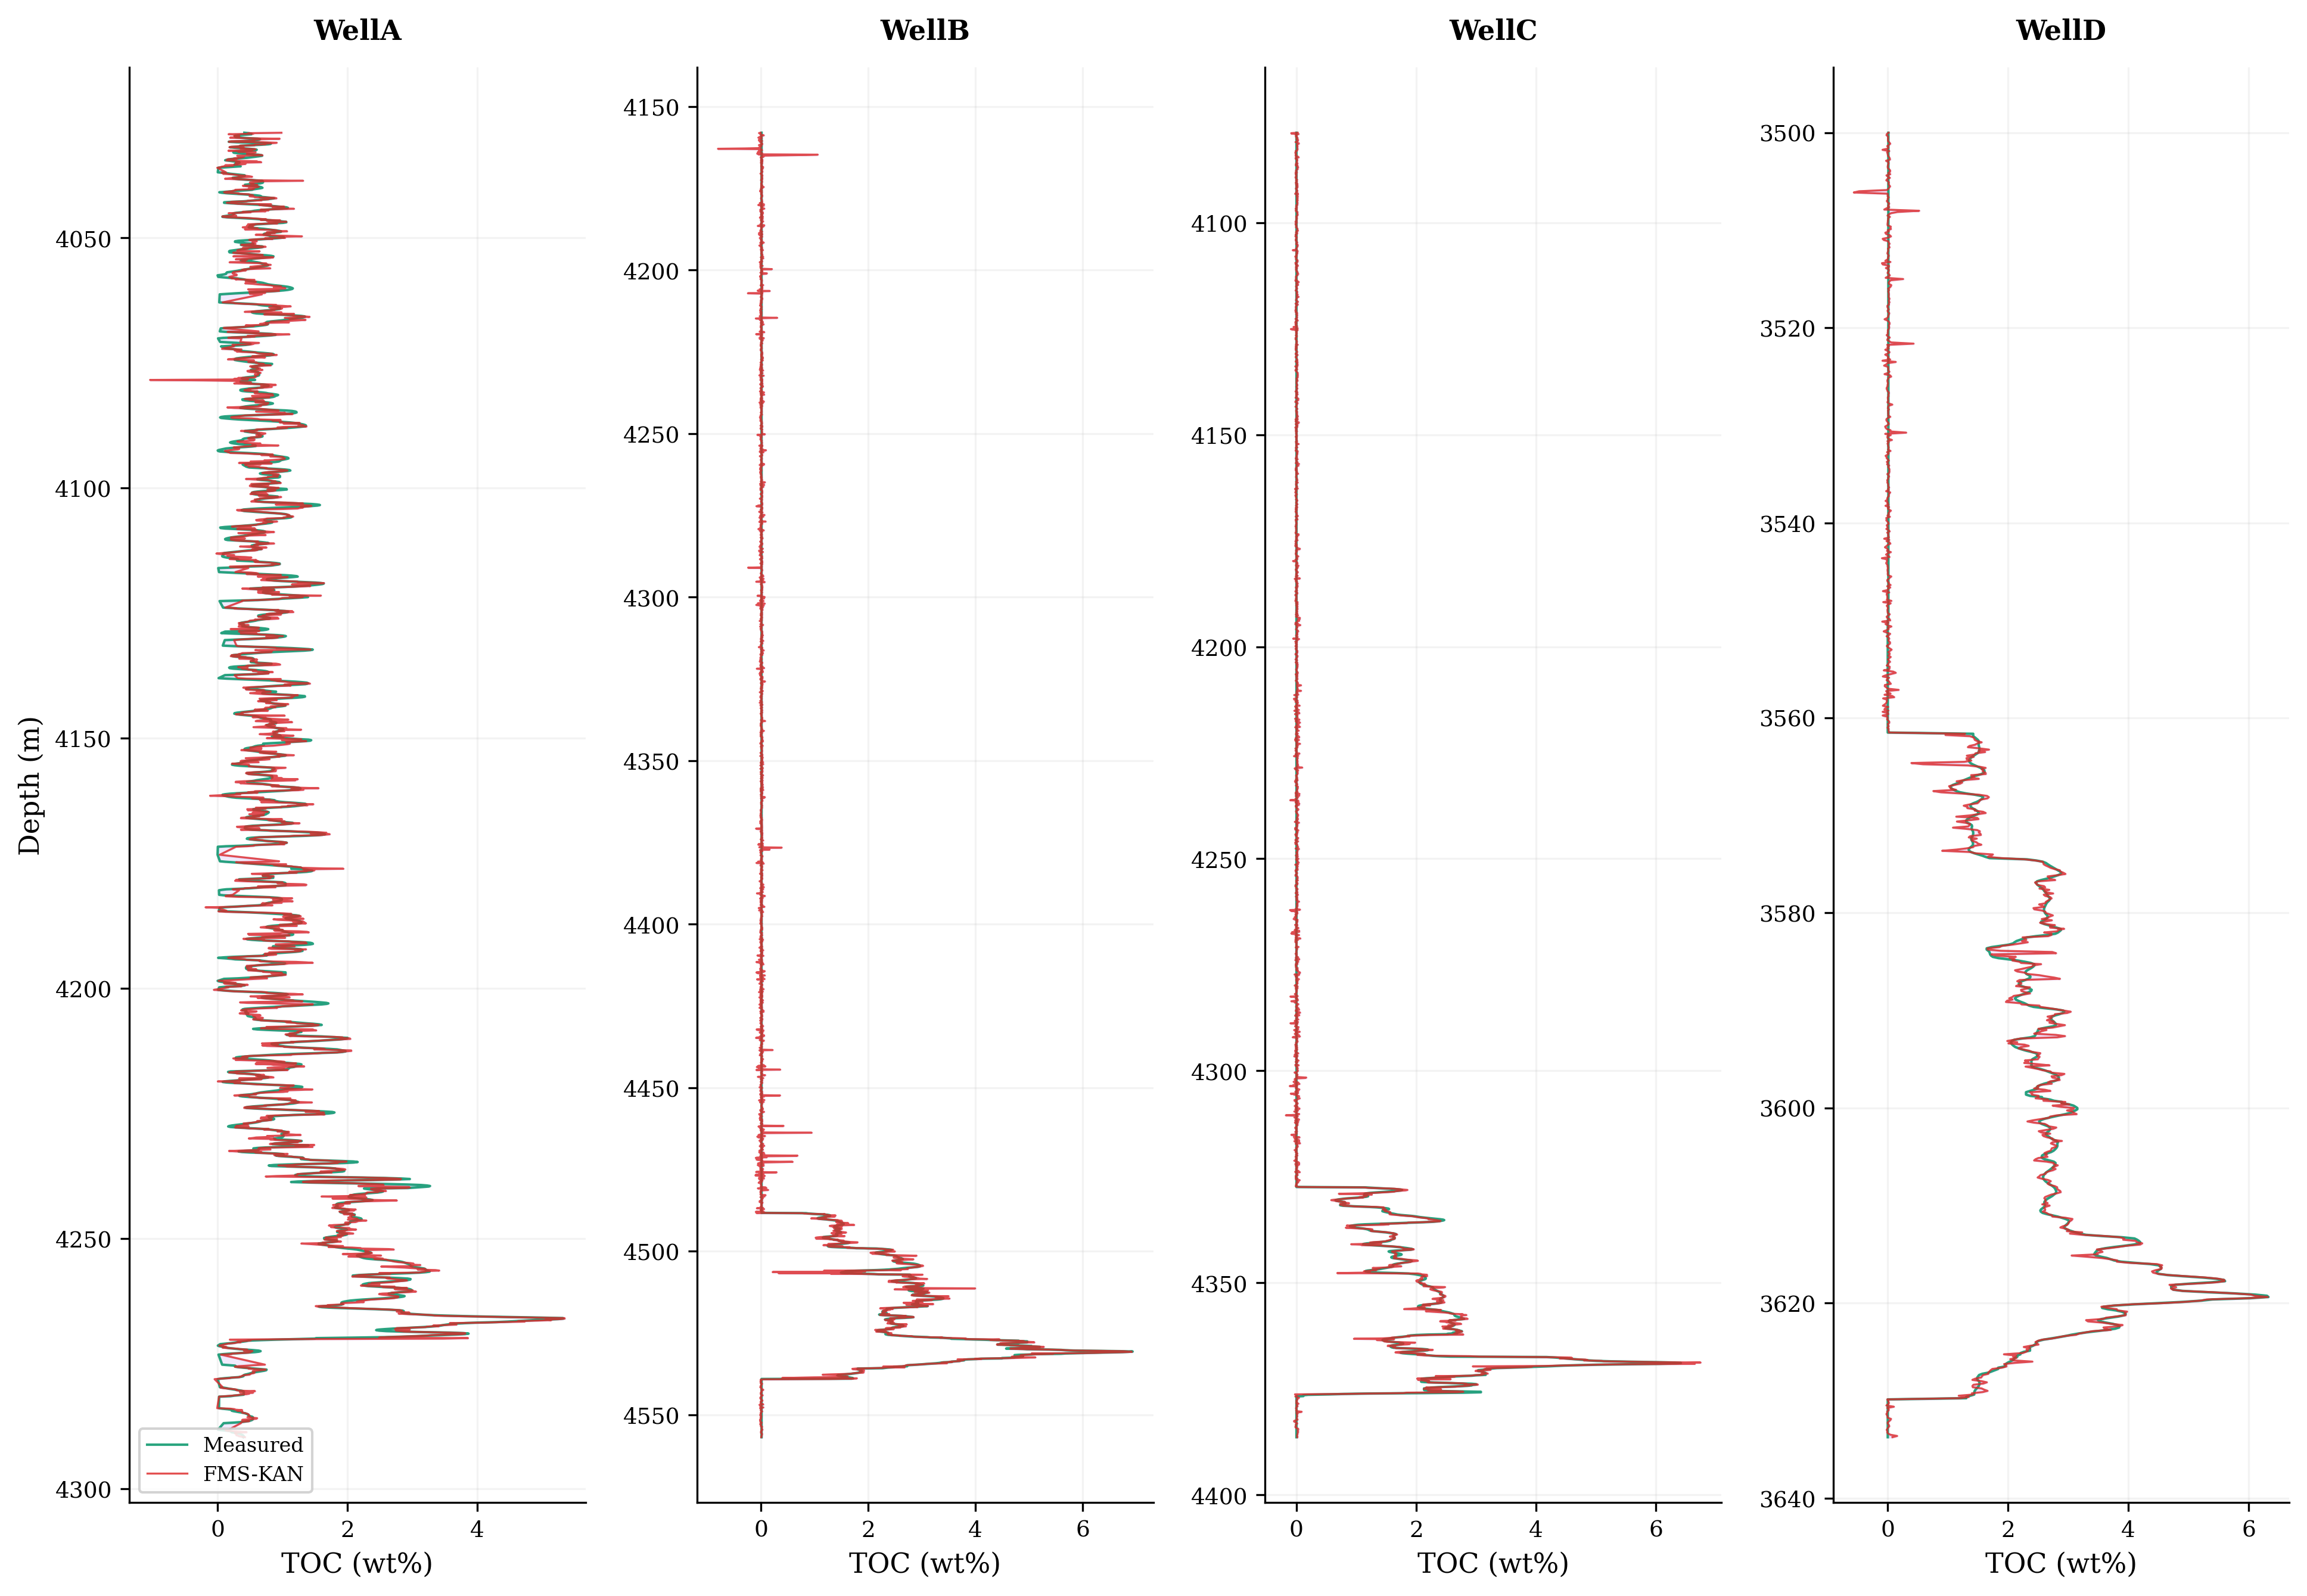
\includegraphics[width=\textwidth]{fig_depth_b_TOC.png}
  \caption{总有机碳（TOC）深度剖面对比}
  \label{fig:depth_toc}
\end{figure*}
\begin{figure*}[htbp]
  \centering
  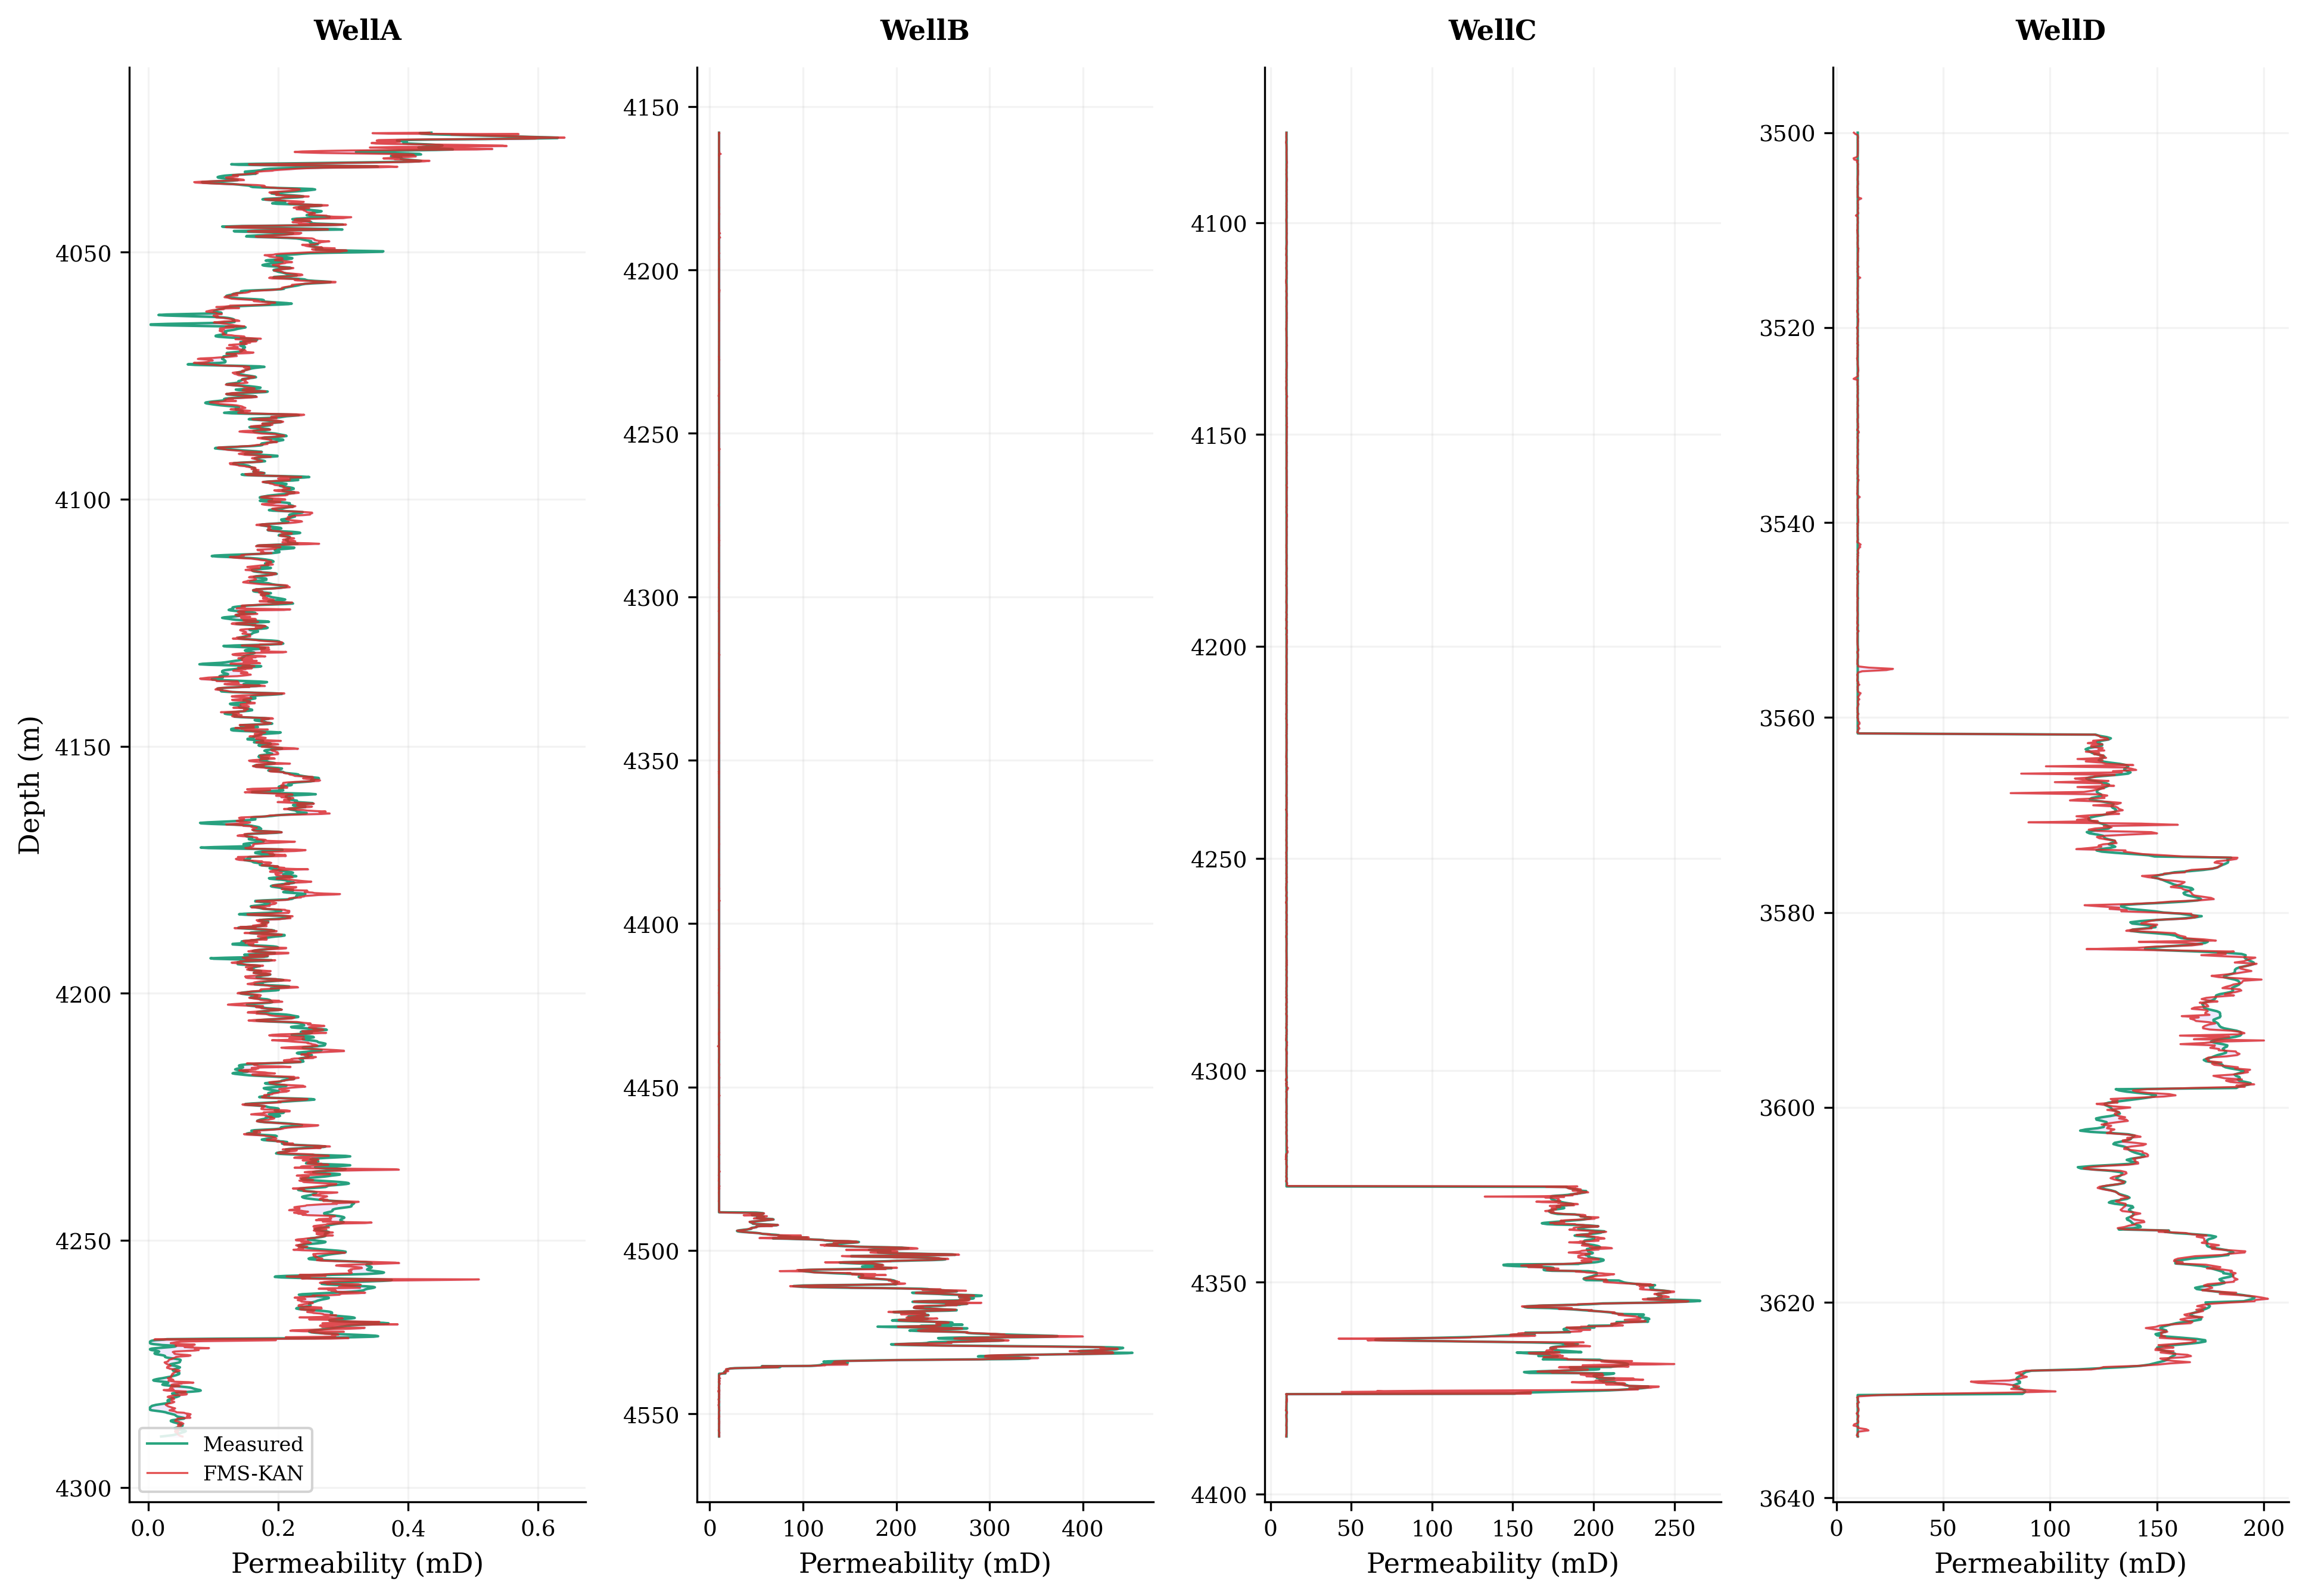
\includegraphics[width=\textwidth]{fig_depth_c_PERM.png}
  \caption{渗透率（PERM）深度剖面对比}
  \label{fig:depth_perm}
\end{figure*}

\subsection{可解释性分析}

图~\ref{fig:feature}展示各目标的特征重要性热力图：声波（DTC、DTS）与密度（DEN）在各目标中均位列前排，与岩石物理理论一致；自然伽马、井斜等对地应力，能谱与电阻率对总有机碳、渗透率也表现出各自贡献。该重要性排序（基于随机森林）用于识别各参数的物理主控曲线，并与提取公式的主导变量相互印证；图中仅含12个原始测井字段。

\begin{figure}[htbp]
  \centering
  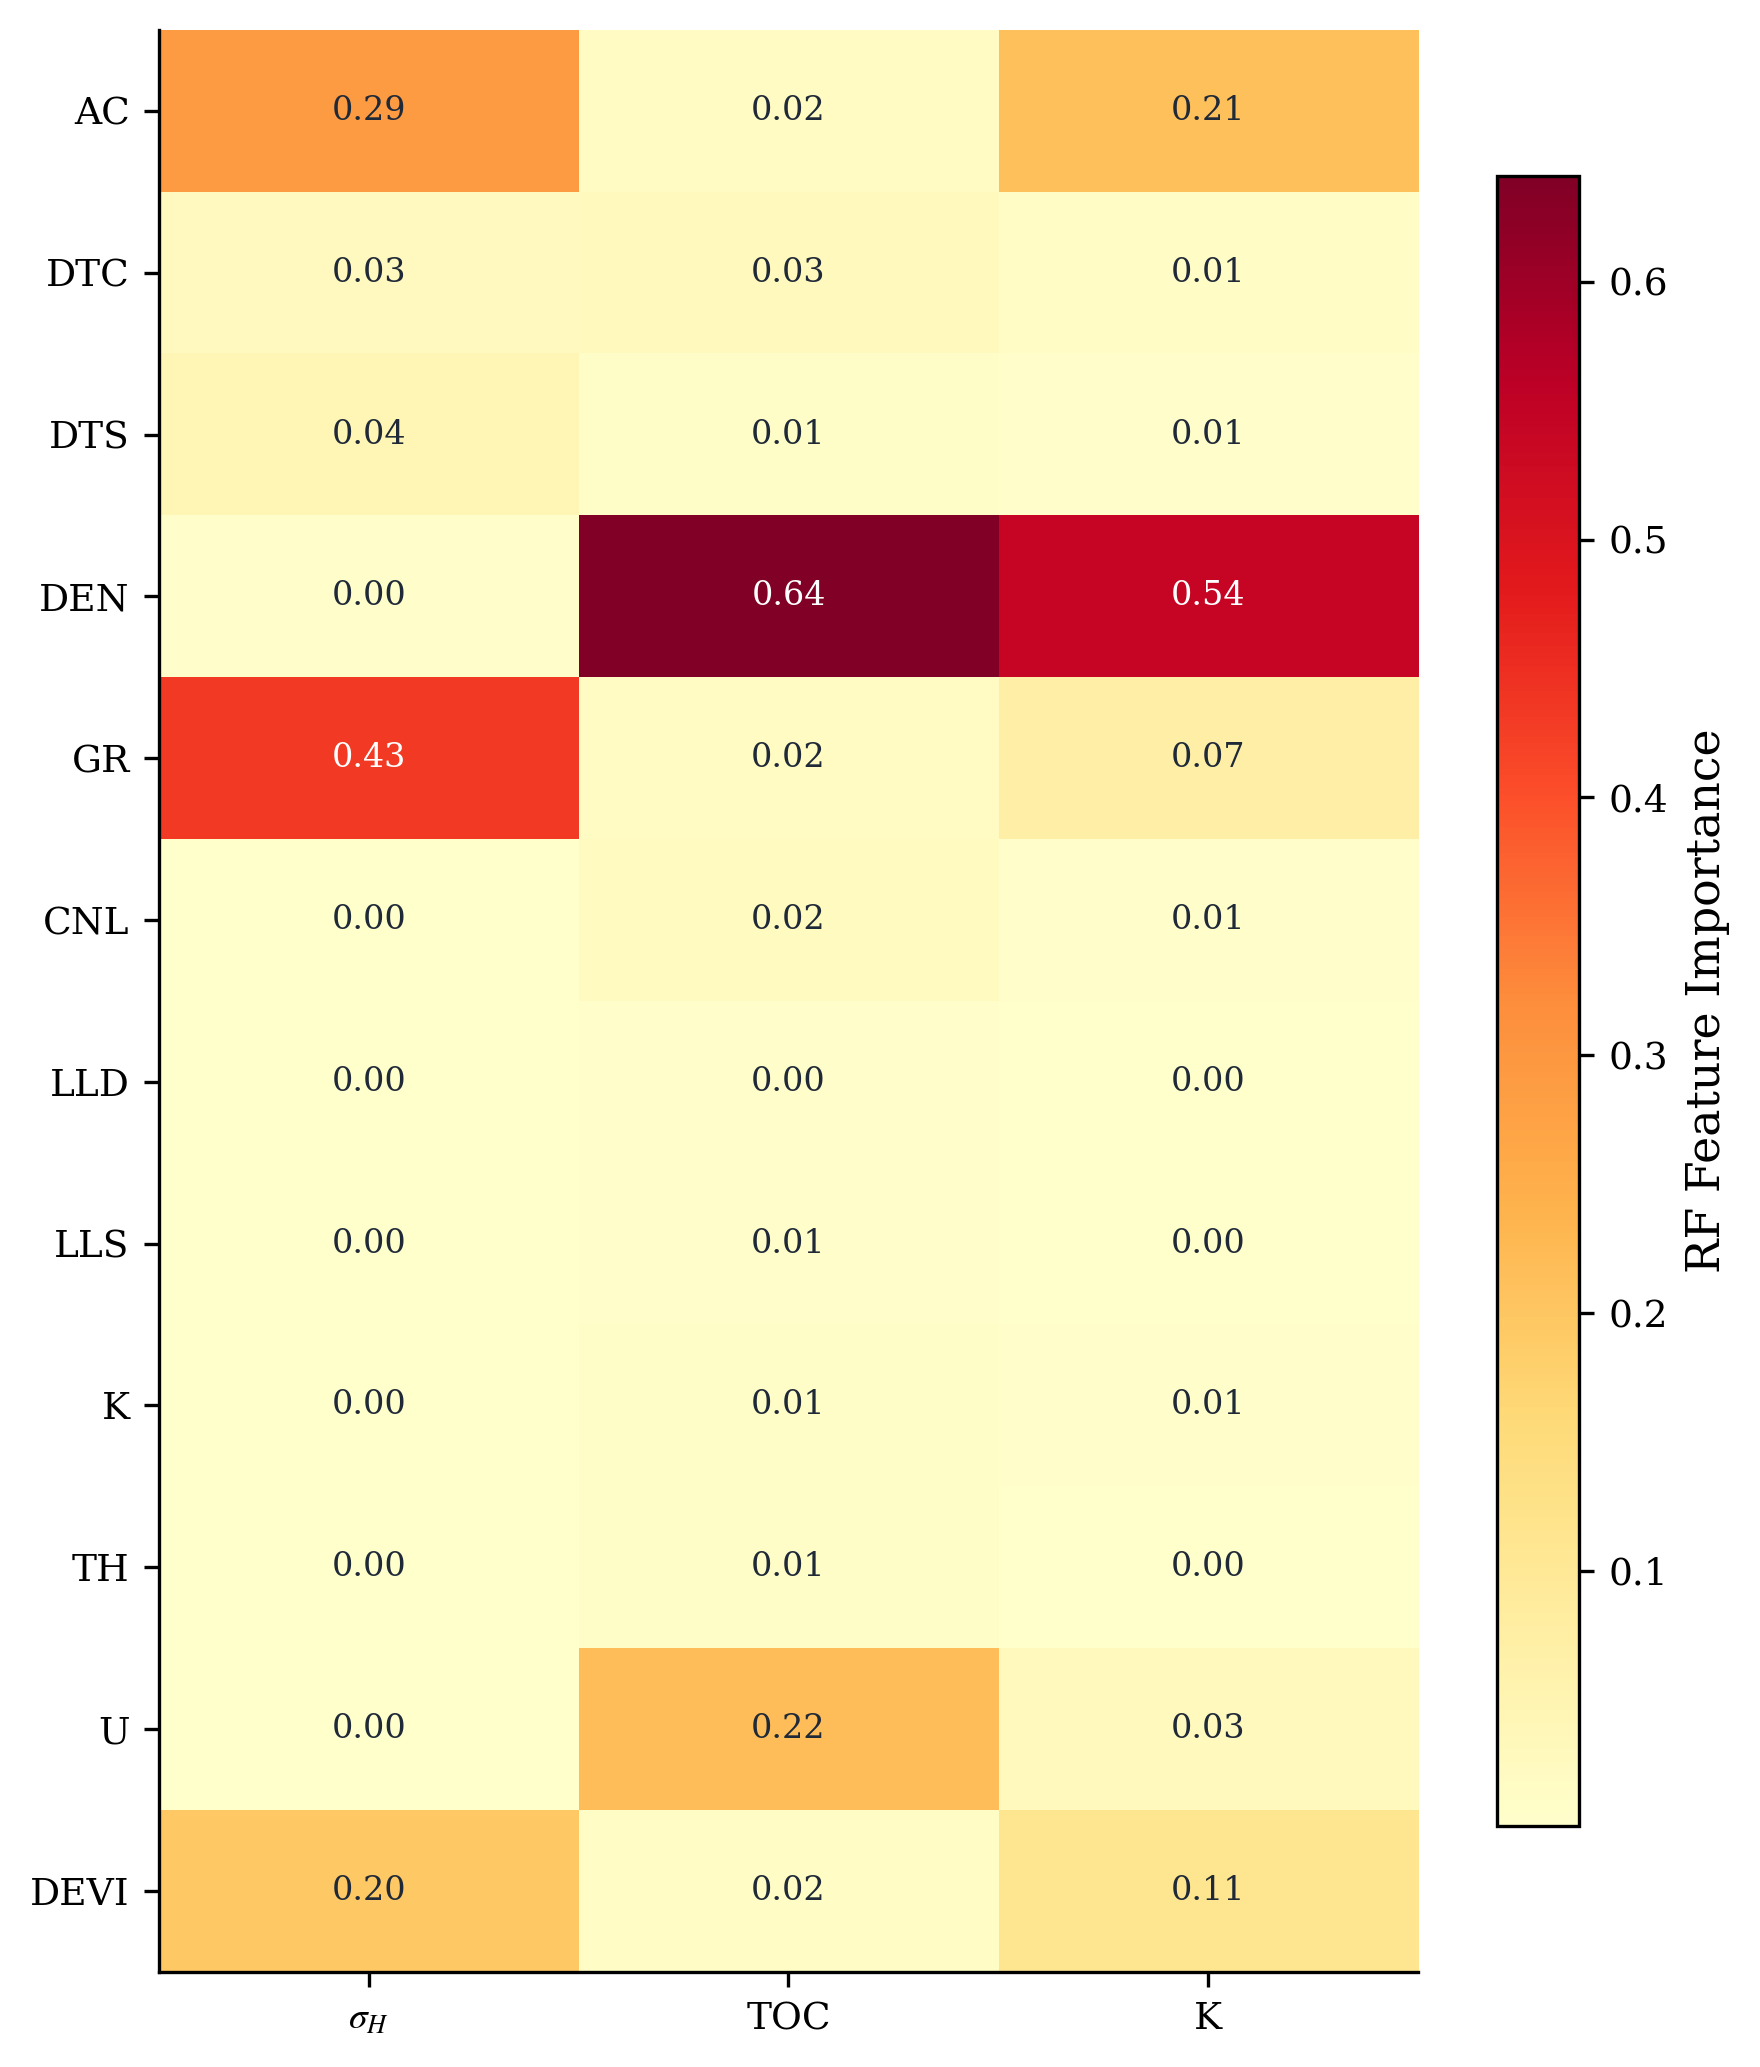
\includegraphics[width=\linewidth]{fig_feature_heatmap.png}
  \caption{各目标特征重要性热力图（随机森林，12个原始测井字段）}
  \label{fig:feature}
\end{figure}

\subsection{知识发现：参数预测公式}

FMS-KAN通过对学习到的B-spline激活函数剪枝与符号简化提取解析预测公式。区别于以往做法，本文公式直接对最终FMS-KAN本身（同架构、同12特征）原地剪枝、符号化得到，因此可解释公式与精度评估来自同一模型；符号化采用数值稳健的函数库（$x,x^2,x^3,\tanh$）。以总有机碳（TOC）为例，符号化得到一组简洁的线性主控式（式中各特征均为 z-score 标准化值，以上标 $*$ 标记）：
\begin{equation}
\begin{aligned}
  \text{TOC} \approx{}& 0.419\,\text{U}^{*} - 0.415\,\text{DEN}^{*} + 0.249\,\text{DTC}^{*} \\
  &{} - 0.285\,\text{CNL}^{*} + 0.075\,\text{GR}^{*} + 0.052\,\text{TH}^{*} \\
  &{} - 0.058\,\text{DEVI}^{*} - 0.056\,\text{DTS}^{*} - 0.044\,\text{K}^{*} \\
  &{} - 0.042\,\text{LLS}^{*} + 0.005\,\text{LLD}^{*} - 0.002\,\text{AC}^{*}
\end{aligned}
\end{equation}
该式在测试集上保持 $R^2=0.837$，相对符号化前的连续模型（$0.973$，见表~\ref{tab:main}）为可接受的精度损失，换来了可直接现场计算、可物理审阅的显式形式；其主导变量（铀U、密度DEN、声波DTC、中子CNL）与图~\ref{fig:feature}的随机森林特征重要性一致，形成交叉印证。对最大水平主应力（SHMAX）与渗透率（PERM），连续FMS-KAN精度很高（$R^2$ 分别为 0.996、0.974，见表~\ref{tab:main}），但在本文简洁函数库下其紧凑闭式的符号拟合不稳定（SHMAX 易退化为含高阶交互的冗长表达、PERM 符号化 $R^2<0$），故如实保留其 KAN 数值模型而不强行给出解析式。这也反映了不同目标"可解析化难度"的显著差异，是当前方法的一个诚实边界。

\section{讨论}

本研究结果对测井参数智能解释具有若干启发。其一，从"精度—可解释性"权衡看，FMS-KAN在总有机碳与渗透率上超越全部黑盒、在最大水平主应力上与最强黑盒持平，提示在中等样本量、强物理先验的测井场景中，将可学习激活函数与领域知识结合有望打破"高精度必黑盒"的假设——可解释性不必以牺牲精度为代价。其二，配对消融显示多尺度细化在最大水平主应力与总有机碳上带来明显提升、在渗透率上与单尺度相当，说明其增益与目标的多尺度特性相关，而非对所有目标同等作用。其三，FMS-KAN提取的解析公式使预测逻辑可被审阅验证，且公式与精度评估来自同一模型；随机森林特征重要性与公式主导变量的一致性进一步增强了结果可信度，这在安全性要求极高的石油工程中尤为重要。本研究仍存在局限：数据来自单一油田，跨盆地泛化尚需验证；仅验证3个代表性参数。未来工作可引入跨井迁移学习，并探索将岩石力学理论方程作为硬约束嵌入训练的物理信息KAN混合建模，以提升外推可靠性。

\section{结论}

针对测井参数预测中"精度与可解释性难以兼顾"的核心矛盾，本文提出特征引导多尺度KAN方法（FMS-KAN），以多分辨率B-spline刻画多尺度特征、以树模型特征重要性引导主控变量分析、以"先连续后离散"策略对同一模型提取解析公式。在某油田4口探井、最大水平主应力/总有机碳/渗透率3个目标上，FMS-KAN取得测试集 $R^2$ 均值 0.981，在总有机碳与渗透率上超越全部黑盒、在最大水平主应力上与最强黑盒基本持平，全面优于传统方法，并在配对消融下相对单尺度标准KAN稳定提升 +0.014。在保持主流黑盒精度的同时提供显式可解释公式，FMS-KAN为测井参数的连续剖面预测提供了一种兼具数据驱动精度与物理可解释性的新范式。

\section*{数据可用性声明}
本研究所用测井数据由数据提供方授权使用。原始数据经与数据提供方沟通确认后进行了标准化质量控制，包括剔除哨兵/缺失记录、依据物理取值范围剔除不合格记录及经核实的占位型异常记录。公开代码仓库中提供经脱敏、随机抽取的部分样本子集用于方法复现；完整数据受数据提供方限制不公开。

\begin{thebibliography}{25}
\bibitem{ref1} Cranmer M, et al. Discovering symbolic models from deep learning with inductive biases. NeurIPS, 2020, 33: 17429-17442.
\bibitem{ref2} Liu Z, et al. KAN: Kolmogorov-Arnold Networks. arXiv:2404.19756, 2024.
\bibitem{ref3} Kolmogorov A N. On the representation of continuous functions of many variables. Dokl. Akad. Nauk SSSR, 1957, 114(5): 953-956.
\bibitem{ref4} Arnold V I. On functions of three variables. Dokl. Akad. Nauk SSSR, 1957, 114(4): 679-681.
\bibitem{ref5} Liu Z, et al. KAN 2.0: Kolmogorov-Arnold Networks meet science. arXiv:2408.10205, 2024.
\bibitem{ref6} Chen T, Guestrin C. XGBoost: a scalable tree boosting system. KDD, 2016: 785-794.
\bibitem{ref7} Lundberg S M, Lee S I. A unified approach to interpreting model predictions. NeurIPS, 2017: 4765-4774.
\bibitem{ref8} de Boor C. A Practical Guide to Splines. Revised ed. Springer, 2001.
\bibitem{ref9} Zoback M D. Reservoir Geomechanics. Cambridge University Press, 2007.
\bibitem{ref10} Fjaer E, et al. Petroleum Related Rock Mechanics. 2nd ed. Elsevier, 2008.
\bibitem{ref11} Eaton B A. The equation for geopressure prediction from well logs. SPE, 1975: SPE-5544-MS.
\bibitem{ref12} Biot M A. General theory of three-dimensional consolidation. J. Appl. Phys., 1941, 12(2): 155-164.
\bibitem{ref13} Passey Q R, et al. A practical model for organic richness from porosity and resistivity logs. AAPG Bull., 1990, 74(12): 1777-1794.
\bibitem{ref14} Breiman L. Random forests. Machine Learning, 2001, 45(1): 5-32.
\bibitem{ref15} Schmidt M, Lipson H. Distilling free-form natural laws from experimental data. Science, 2009, 324(5923): 81-85.
\bibitem{ref16} Zoback M D, et al. Determination of stress orientation and magnitude in deep wells. Int. J. Rock Mech. Min. Sci., 2003, 40(7-8): 1049-1076.
\bibitem{ref17} Chang C, et al. Empirical relations between rock strength and physical properties. J. Pet. Sci. Eng., 2006, 51(3-4): 223-237.
\bibitem{ref18} Ameen M S, et al. Predicting rock mechanical properties of carbonates from wireline logs. Mar. Pet. Geol., 2009, 26(4): 430-444.
\bibitem{ref21} Timur A. An investigation of permeability, porosity, and residual water saturation relationships. SPWLA, 1968.
\bibitem{ref22} Jaeger J C, et al. Fundamentals of Rock Mechanics. 4th ed. Blackwell, 2007.
\bibitem{ref23} Ulusay R, Hudson J A. The Complete ISRM Suggested Methods. Springer, 2015.
\bibitem{ref24} Bozorgasl Z, Chen H. Wav-KAN: Wavelet Kolmogorov-Arnold Networks. arXiv:2405.12832, 2024.
\bibitem{ref25} Shukla K, et al. A comprehensive comparison between MLP and KAN. arXiv:2406.02917, 2024.
\end{thebibliography}

\end{document}
